\chapter{Sistemas PAD para ABC \textit{<<Segregated Two Step>>}}\label{ch:EVALUACIONACION_TOPOLOGIAS}

A lo largo de este capítulo se describe el método \GLS{PAD} para sistemas \GLS{ABC} \textit{<<Segregated Two Step>>}, presentado en \textit{$14$th International Conference on Security and Cryptography, SECRYPT 2017}  \cite{del2017face}. La solución propuesta se diseñó e implantó en los sistemas pilotos \GLS{ABC} del proyecto a \GLS{ABC4EU}. En la Sección \ref{sec:SisABC4EU} se describe la operativa de este tipo sistemas que al tratarse de sistemas \textit{<<Segregated Two Step>>} requieren de dos verificaciones biométricas, es decir dos puntos débiles para ataques de presentación (para ver mas información sobre este tipo de sistemas ver Sección \ref{subsec:Topologias}). En el la Sección \ref{sec:PADSegregado} se describe el método \GLS{PAD} propuesto. En el apartado \ref{sec:ExperimentosABC4EU} se describen los experimentos realizados y a continuación los resultados obtenidos se detallan en la Sección \ref{sec:ResultadosABC4EU}. 


%%%%%  ABC de ABC4EU %%%%%%%%
\section{Sistemas ABC4EU}\label{sec:SisABC4EU}

\begin{figure}
\centering
    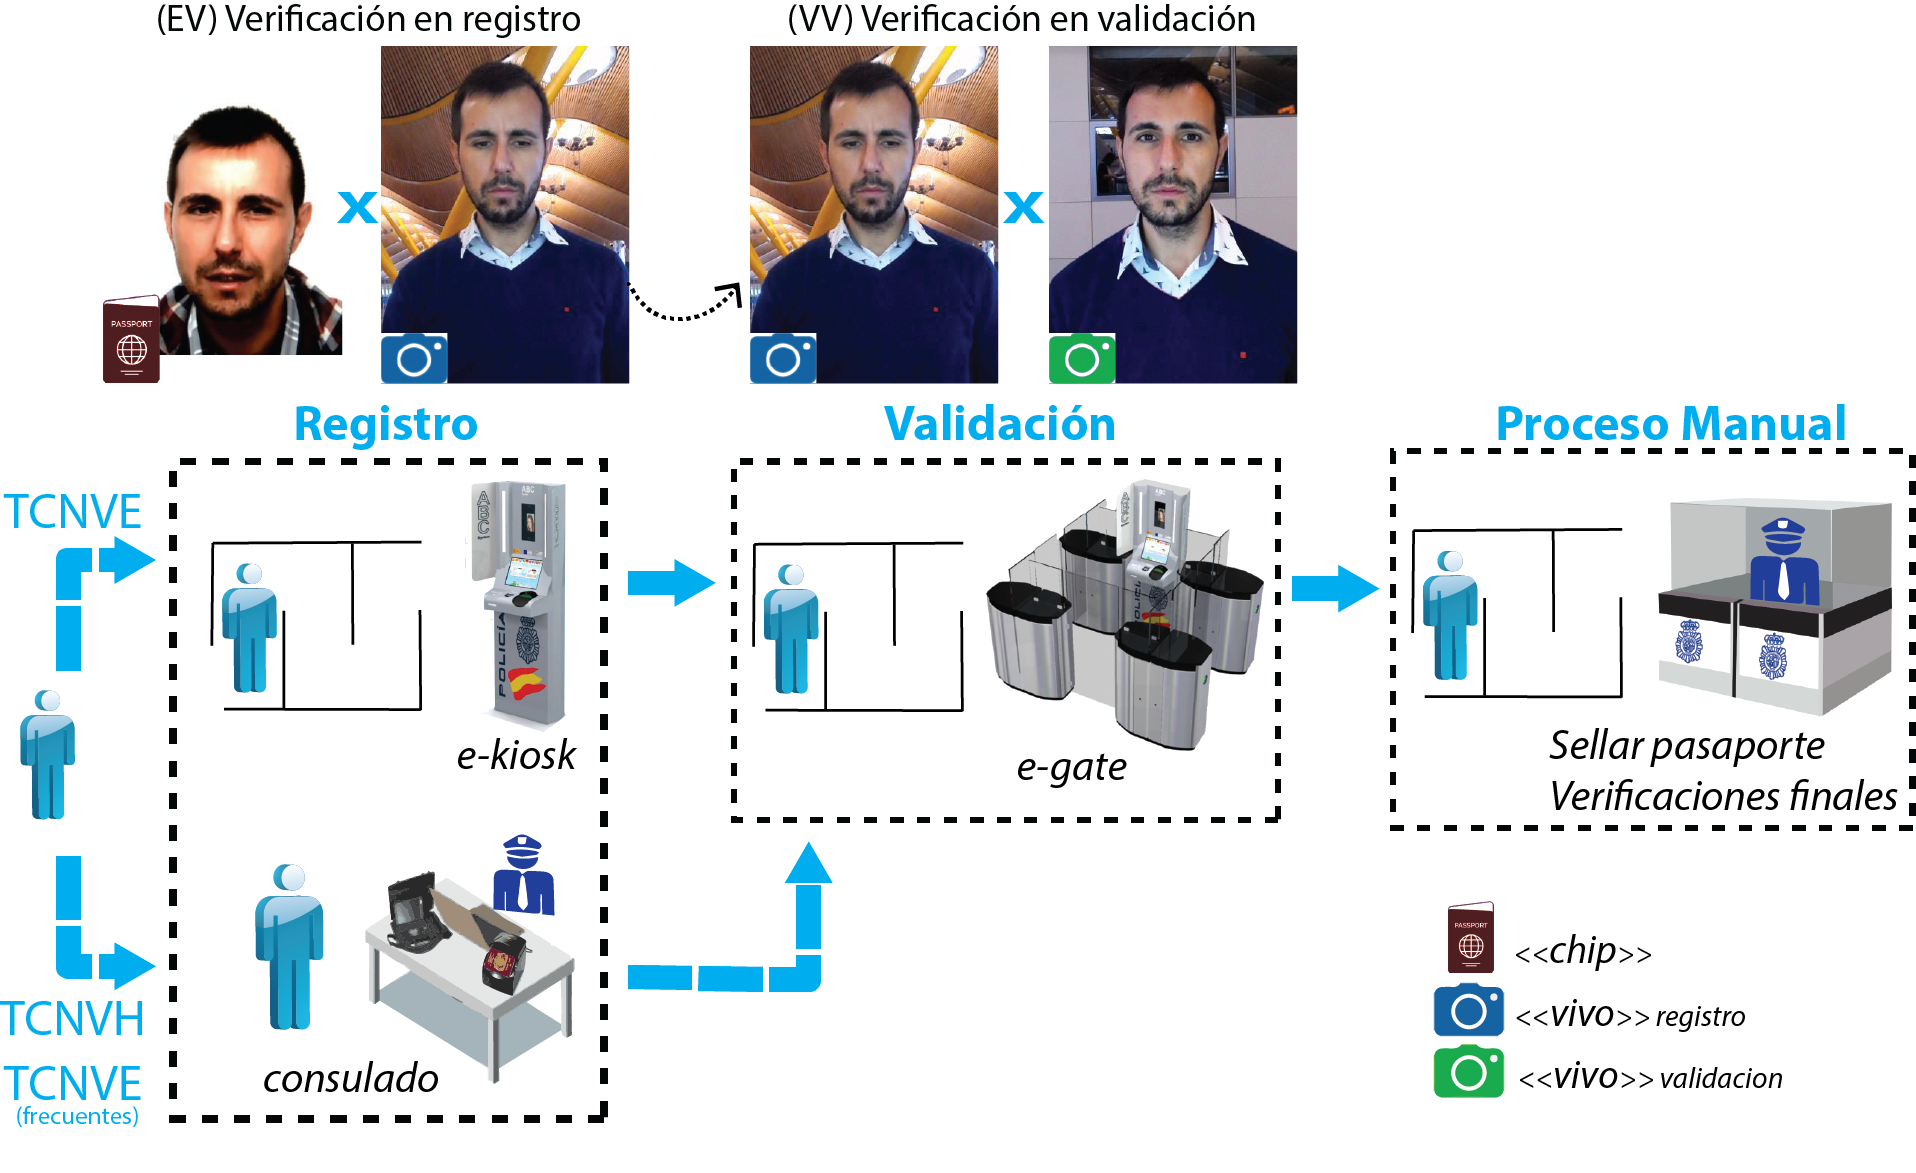
\includegraphics[width=\textwidth]{ch-sistemasABC/images/ch-evaluacion_topologias/ARQUIETECTURA_ABC_ABC4UE.png}
    \caption{Esquema de \GLS{ABC4EU}.}
    \label{fig:EsquemaABC4EU}
\end{figure}

Los sistemas \GLS{ABC4EU} son sistemas \GLS{ABC} \textit{<<Segregated Two Step>>}, con una etapa de registro \GLS{RTP} que puede realizarse de forma remota, para las pruebas se realizo de forma presencial en un \gls{e-kiosk} y una etapa de validación \GLS{EES} que se realiza en un \gls{e-gate} al cruzar la frontera (ver Fig. \ref{fig:EsquemaABC4EU}). 

\subsection{Registro: \textit{e-kiosk}}

\color{blue}Los \GLS{ABC} analizados son el prototipo de sistema propuesto en el proyecto \GLS{ABC4EU} por lo que ha sido posible evaluar el sistema en varios cruces de frontera reales durante la implantación de los pilotos del proyecto.
El proyecto europeo \GLS{ABC4EU} propone sistemas \GLS{ABC} para las fronteras de la \GLS{EU}. Los sistemas que propone es del tipo \GLS{ABC} \textit{<<Segregated Two Step>>}.\color{black}

En el registro el viajero presenta su \Gls{eMRTD}, el sistema lee sus datos del \gls{chip}. El proceso contrasta los datos del viajero con las bases de datos correspondientes, y certifica que el viajero es el verdadero titular del documento. Para ello, el sistema valida los datos biométricos \gls{chip} almacenados en el documento con los datos biométricos capturados en ese momento del registro (\gls{vivo registro}).

Cuando el proceso de registro ha realizado todos las comprobaciones con éxito, el sistema almacena los datos del viajero registrado durante un período limitado de tiempo, dependiendo del tipo de viajero. Durante este periodo, el viajero puede acceder a la \gls{e-gate} y cruzar la frontera si supera la etapa de validación.

\color{blue}Este sistema tiene operativas distintas dependiendo del tipo de viajeros: Si necesitan un visado o son viajeros frecuentes.

La operativa se compone de dos etapas el \GLS{RTP} y \GLS{EES} que llamaremos registro y validación.

Cada una de estas etapas tiene una verificación facial: en registro la verificación se realiza en entre la imagen de \gls{chip} y una imagen capturada en es momento \gls{vivo registro} y en validación la verificación se realiza entre la imagen \gls{vivo registro} y una nueva imagen que se captura del viajero en la \gls{e-gate} \gls{vivo validacion}. (ver Fig. \ref{fig:EsquemaABC4EU})


Los sistemas\GLS{ABC} \textit{<<Segregated Two Step>>} realizan los procesos \GLS{RTP} y \GLS{EES} en dos dispositivos distintos un \gls{e-kiosk} y una \gls{e-gate} (para más información sobre estos procesos ver Sección \ref{subsec:ArquitecturaLogicaABC}). Cada uno de estos dispositivos tiene un sistema de captura en el que se realiza una verificación facial.

En la etapa de \GLS{RTP} una verificación facial entre el \gls{chip} del pasaporte y una imagen de viajero capturada en el registro (\gls{vivo registro}) y en la etapa \GLS{EES} una verificación entre el \gls{vivo registro} capturado en la etapa anterior y una nueva imagen capturada en ese momento en la \gls{e-gate} (\gls{vivo validacion}).
\color{black}

El sistema considera dos protocolos diferentes dependiendo del tipo de viajero. Por un lado, los viajeros \GLS{TCNVE} que pueden hacer el registro  en el \gls{e-kiosk} al llegar al aeropuerto antes de su viaje. Y por otro lado, los viajeros \GLS{TCNVH}, que no pueden hacer el registro en el aeropuerto y obligatoriamente deben registrarse en el sistema en su consulado antes de la etapa de verificación en el aeropuerto. También, los viajeros \GLS{TCNVE} que sean viajeros frecuentes, pueden registrarse en el sistema, en su consulado y se evitan realizar un registro en cada viaje. 

\subsection{Validación: \textit{e-gate}}

El proceso de validación siempre tiene lugar en la \gls{e-gate} después de la etapa de registro. La etapa de validación consiste en comparar una nueva captura de los datos biométricos del viajero \gls{vivo validacion} con los datos biométricos capturados en la etapa del registro \gls{vivo registro}.

Tanto el los viajeros \GLS{TCNVE} como los viajeros \GLS{TCNVH} deben pasar esta etapa.

%%%%%  PAD SEGREGADO %%%%%%%%
\section{PAD \textit{<<Segregated Two Step>>}}\label{sec:PADSegregado}

\begin{figure}
    \centering
    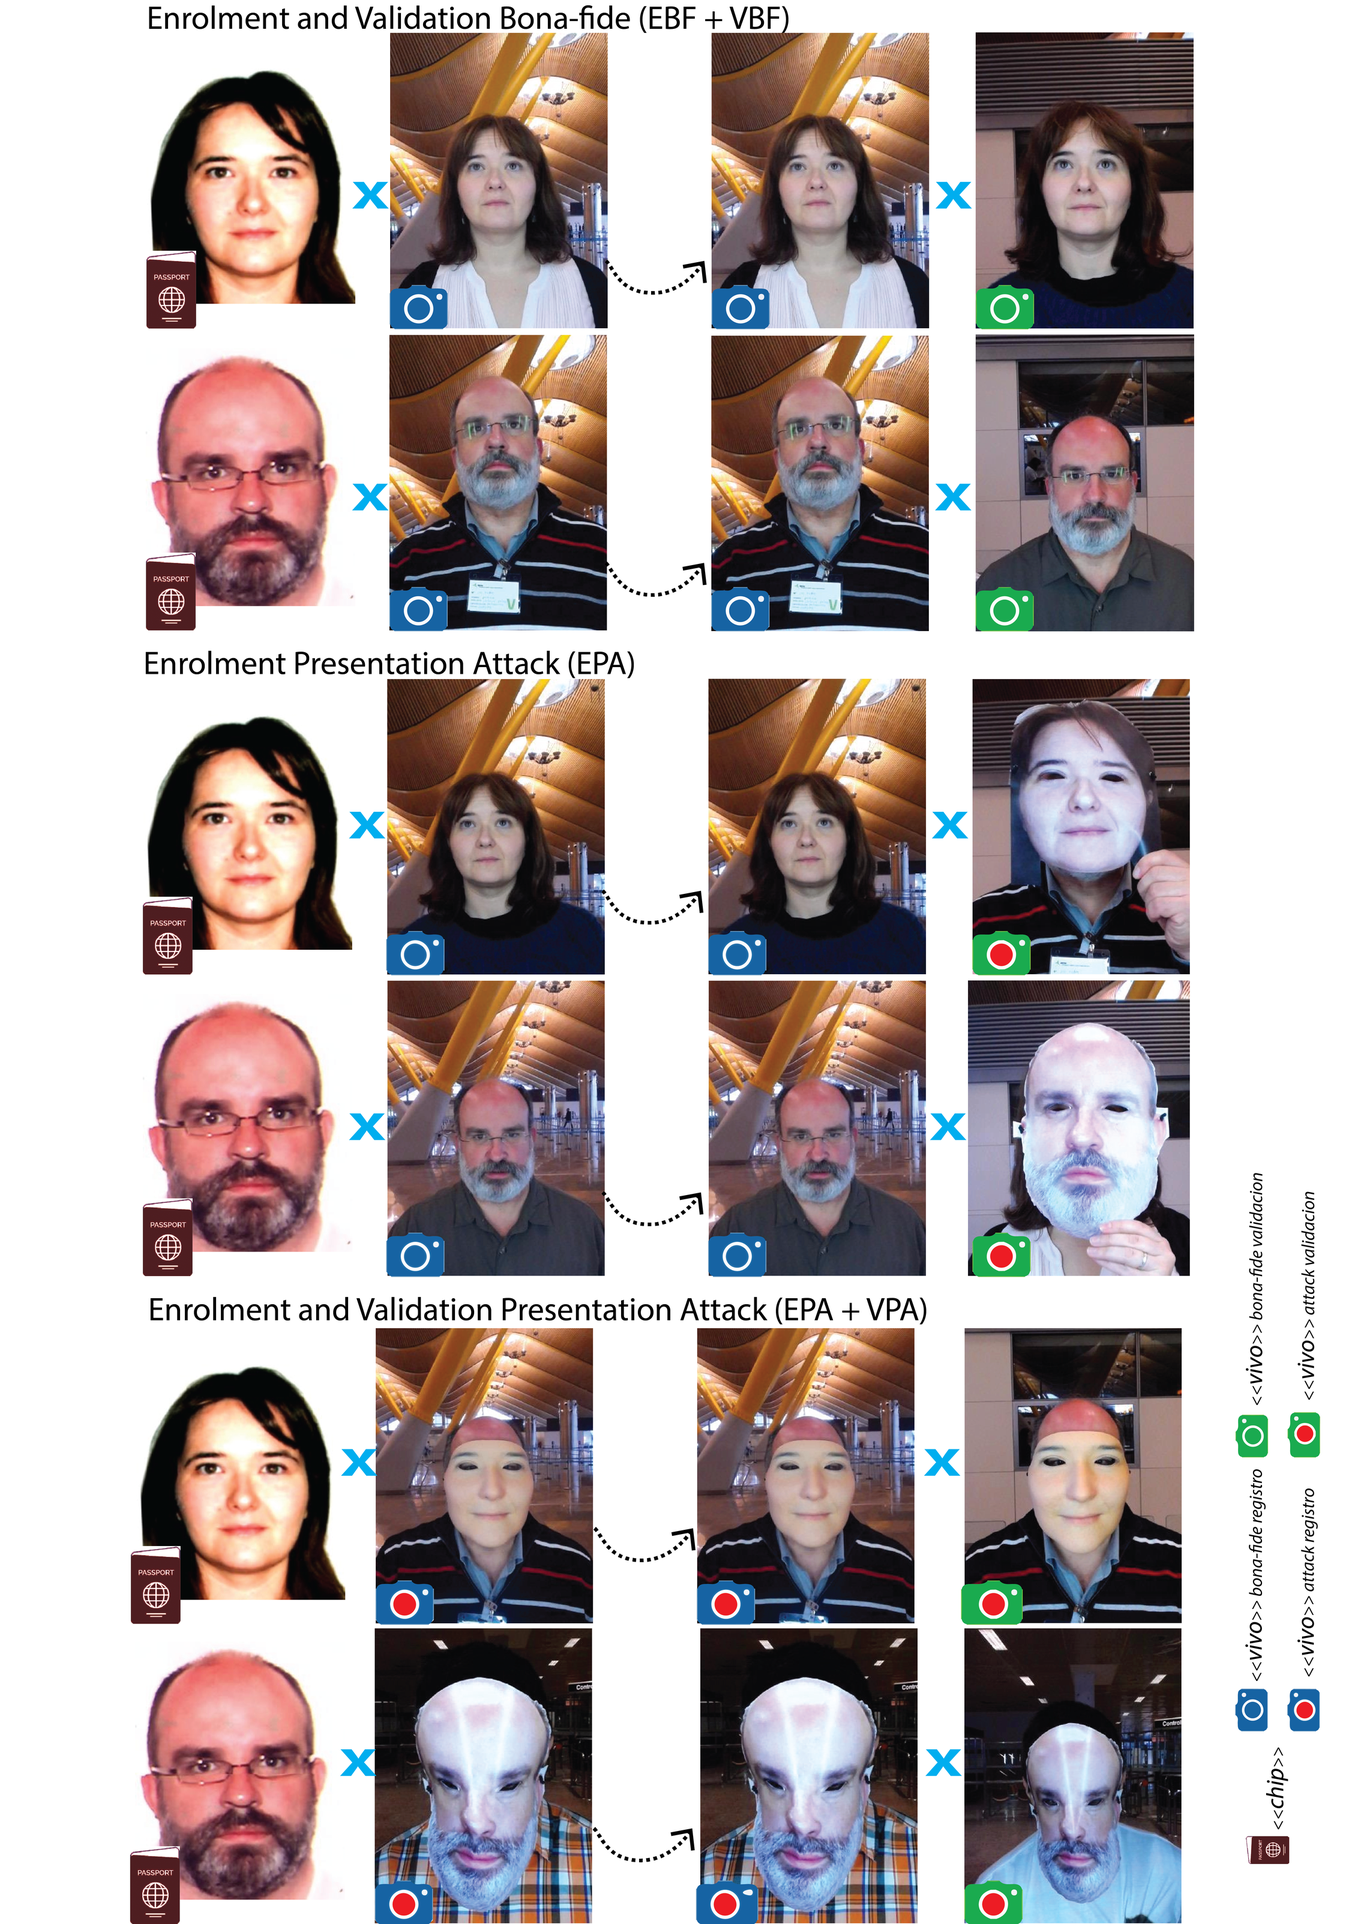
\includegraphics[width=\textwidth]{ch-sistemasABC/images/ch-evaluacion_topologias/ESCENARIOS_VERIFICACION_DOS_PASOS_VER.png}
    \caption{Escenarios de verificación en sistemas \GLS{ABC} \textit{<<Segregated Two Step>>}.}
    \label{fig:escenariosVerifacionABC}
\end{figure}

Los ataques de presentación se producen en la fase de captura a nivel del sensor del subsistema biométrico (Ver Sección \ref{sec:ContextoAtaquesPresentacion}). Como los sistemas \GLS{ABC} del proyecto \GLS{ABC4EU} están organizados en dos etapas segregadas, se realizan dos capturas diferentes: una en el \gls{e-kiosk}, para el registro y la otra en la \gls{e-gate}, para la validación. Esto hace que el sistema tenga dos puntos vulnerables y que sea necesario considerar tres escenarios diferentes para un posible ataque (ver Fig. \ref{fig:escenariosVerifacionABC}).

\begin{itemize}
    \item
    \textit{Enrolment Presentation Attack} (\GLS{EPA}): Cuando el ataque se produce en la etapa de registro. Por ejemplo, un atacante se registra en el sistema con una documentación que pertenece a otra persona tratando de hacerse pasar por el verdadero titular de los documentos.
    \item
    \textit{Verification Presentation Attack} (\GLS{VPA}), Cuando el ataque de presentación se produce en la etapa de verificación. Un el atacante intenta hacerse pasar por un viajero que se ha registrado previamente en el sistema. Por ejemplo, cuando un viajero registrado correctamente pierde o le roban sus documentos entre la etapa del registro y la etapa de verificación. Entonces un atacante usa esos documentos para intentar para pasar la verificación.
    \item
    \textit{Enrolment and Verification Presentation Attack} (\GLS{EPA}+\GLS{VPA}). En este caso se trata de un doble ataque, la suplantación tiene lugar en el momento del registro y en la etapa de verificación, el atacante continúa haciéndose pasar por el verdadero viajero. Por ejemplo, un atacante presenta la documentación de otra persona y se registra con éxito. Y posteriormente, en la etapa de verificación, continúa haciéndose pasar por el verdadero poseedor de la documentos para cruzar la frontera.
\end{itemize}

Estos tres escenarios complican la evaluación del subsistema \GLS{PAD}.

En Fig. X a se pueden ver las curvas \GLS{ROC} de los resultados obtenidos en la verificación facial del registro, con distintos reconocedores faciales \GLSpl{COT}. Y en Fig. X b las curvas con los resultados obtenidos en la verificación  de la validación, con los mismos \GLSpl{COT}. En ambos caso los resultados son muy buenos, algo mejores en validación ya que el en esta etapa la verificación se realiza se realiza entre dos capturas relativamente recientes, \gls{vivo registro} y \gls{vivo validacion}. mientras que en registro la imagen \gls{chip} del pasaporte puede ser muy antigua (los pasaportes tienen distintos periodos de validez).
\color{red}figura con los \textit{score} de dgp de dos empresas que realmente son ABCS\color{black}

Cada uno de las gráficas de la figura Y muestra tres distribuciones de densidad de \textit{scores} obtenidos con uno de los reconocedores \GLSpl{COT} usados en las verificaciones del sistema: la distribución con los \textit{scores} de cruces negativos (en rojo), \textit{scores} de cruces positivos (en verde) y \textit{scores} de cruces de ataque (en azul). En cada una de las gráficas los \textit{scores} de ataque corresponde a cruces con tipo de \GLS{PAI} diferente. Como se puede ver en todas ellas el umbral que serviría para distinguir cruces positivos de cruces negativos (se ha elegido el umbral del \GLS{EER}) hace que los ataques sean considerado como cruces positivos lo que indica que los reconocedores empleados pueden ser engañados fácilmente con casi cualquier tipo de ataque.
\color{red}figura con una matriz de distribuciones, una por ataque los \textit{scores} de dgp de dos empresas que realmente son ABCS\color{black}

Cuando se pone a prueba el sistema con ataques se observa la cantidad de ataques que se cuelan ver tabla \color{red}quizás una tabla con los ataque que se cuelan\color{black} y por eso es imprescindible un sistema de detección de ataques de presentación. En la tabla se puede ver que ataques resultan más peligrosos. Además se puede apreciar que la validación es más sensible a los ataques que el registro. Esto se explica por las imágenes que se usan para realizar cada una de las verificaciones. A la hora de realizar los \GLS{PAI} se suelen usar imágenes mas recientes por lo que \gls{vivo validacion ataque} sera más parecido a \gls{vivo registro} que el propio \gls{vivo registro} a la imagen \gls{chip} del pasaporte.

Se propone un sistema \GLS{PAD} como el descrito en el capitulo \ref{ch:PAD_MULTIATAQUE} tanto para la etapa de registro como para la validación. Primero se entreno con la base de datos de \Gls{FRAV-Attack} (ver \ref{sec:BBDD-FRAV-Attack})  que incluye distintos tipos de ataques y se puso a prueba en los sistemas \GLS{ABC4EU} en un cruce de frontera real (Se pueden ver los datos obtenidos en la etapa de registro y en la etapa de validación).
Posteriormente se volvió a entrenar, esta vez con los datos capturados en el escenario real con los que se construyó un subconjunto de \Gls{FRAV-ABC-Attack} con imágenes \gls{vivo registro} e imágenes \gls{vivo validacion} (ver \ref{subsec:FRAV-ABC-ATTACK-DOS_PASOS}). Como era de esperar Los resultados del sistema entrenado con imágenes capturadas en el propio sistema mejoran mucho.


%% EXPERIMENTOS %%%%
\section{Experimentos realizados}\label{sec:ExperimentosABC4EU}

Los sistemas \GLS{ABC4EU} capturan la huella dactilar y una imagen de la cara en el sistema biométrico subsistema. Algunos estudios se han centrado en la verificación dactilar con este tipo de sistemas  \cite{donida2016emerging}, pero este estudio se centra en el reconocimiento facial por dos razones. Por un lado, la imagen de la cara es la única biométrica referencia obligatoria en todos pasaportes en el mundo (en la zona \Gls{Schengen} también el huellas dactilares de la mano izquierda). Y por otro lado, la cara es un rasgo que, en caso de error un agente siempre puede contrastar la información con una fácil inspección visual. Los experimentos realizados analizan los ataques en el registro (\GLS{EPA}) y en la validación (\GLS{VPA}), ambos de forma aislada aislamiento.

Para el registro, se emplearon pasaportes originales y todos los \GLS{PAI} se construyeron con características biométricas de $9$ propietarios legítimos de esos pasaportes. Así, cada \gls{chip bona-fide} se verificó con un \gls{vivo bona-fide} y con $6$ \gls{vivo ataque} con diferentes \GLS{PAI}. 

En la validación, sólo los casos en los que el registro se ha hecho con un \gls{bona-fide} se utilizan presentaciones. De esta manera, una presentación \gls{bona-fide} La presentación (\gls{vivo registro}) se cruza contra una presentación de \gls{bona-fide} (muestra \gls{vivo validacion} y contra 6 ataques con diferentes \GLSpl{PAI}.

El \GLS{PAD} devuelve la probabilidad de que la presentación sea un \gls{bona-fide}.

Para verificar la integridad del sistema contra el y analizar los datos obtenidos por el \GLS{PAD}, se han calculado las curvas \GLS{DET} con el resultado  obtenido de \GLS{APCER} y \GLS{BPCER}. 

Por razones de seguridad (el piloto fue realizado en una zona crítica con una frontera real cruce), la cantidad de sujetos de prueba era limitada. Esta restricción es la razón por la que se ha reducido relativamente el número de número de algunos de los ataques Durante la etapa de registro, véase el cuadro $2$, $61$ se hicieron presentaciones con $6$ viajeros diferentes, teniendo en cuenta los intentos de presentaciones de buena fe y ataques con los diferentes \GLS{PAI}. En la validación, se hicieron $93$ presentaciones en total, pero vamos a sólo usan 48, aquellos en los que se hizo el registro con una presentación \gls{bona-fide}. Se han ignorado el escenario de doble ataque (\GLS{EPA}+\GLS{VPA}).

%%%%%%%%%%%% RESULTADOS %%%%%%%%%%%%%%%%%%%%%%%%
\section{Resultados}\label{sec:ResultadosABC4EU}

\begin{table}
\centering
\begin{tabular}{|l|c|c|}
\hline
\GLS{PAI} & \GLS{D-EER} (registro) & \GLS{D-EER} (verificación) \\ \hline
\textbf{Foto} & $0.2000$ & $0.2071$ \\ \hline
\textbf{Máscara} & $0.0333$ & $0.2071$ \\ \hline
\textbf{Pantalla} & $0.1505$ & $0.1714$  \\ \hline
\textbf{Máscara $3$D} & $0.0000$ & $0.0000$  \\ \hline
\textbf{Morphing} & $0.0000$ & $0.5000$  \\ \hline
\textbf{Camiseta} & $0.2583$ & $0.0000$  \\ \hline
\textbf{Todos los \GLSpl{PAI}} & $0.1210$ & $0.2106$ \\ \hline
\end{tabular}
\caption{Error de detección \GLS{D-EER} obtenido con cada uno de los \GLS{PAI} en la etapa de registro y etapa de verificación.}
\label{tab:EPCERRegistroVerificacion}
\end{table}


\begin{figure}
\centering
    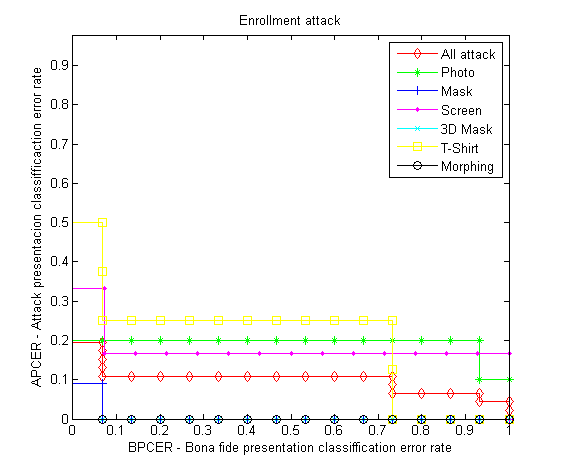
\includegraphics[width=1\textwidth]{ch-sistemasABC/images/ch-evaluacion_topologias/APCER_BPCER_CURVE_ENROLMENT.png}
    \caption{Curva \GLS{DET} con \GLS{APCER}-\GLS{BPCER} en la etapa de registro (Escenario \GLS{EPA}).}
    \label{fig:APCERBPCERRegistro}
\end{figure}

\begin{figure}
\centering
    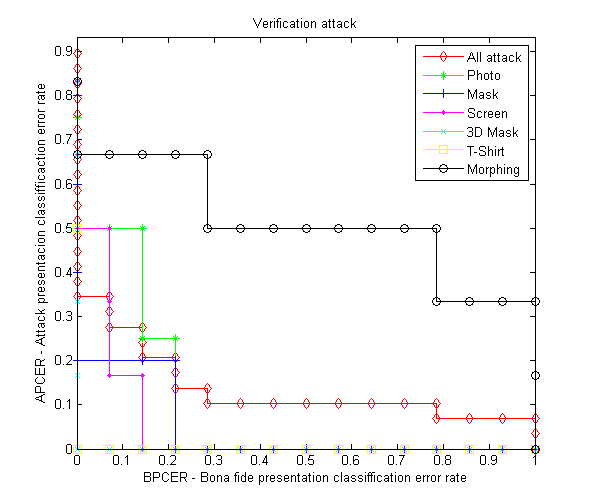
\includegraphics[width=1\textwidth]{ch-sistemasABC/images/ch-evaluacion_topologias/APCER_BPCER_CURVE_IN_THE_VERIFICACION.png}
    \caption{Curva \GLS{DET} con \GLS{APCER}-\GLS{BPCER} en la etapa de registro (Escenario \GLS{VPA}).}
    \label{fig:APCERBPCERVerificacion}
\end{figure}

\color{blue}Se presentan los resultados de las dos verificaciones faciales que se realizan: Una la etapa de registro y otra en la etapa de cruce. También se analiza la resistencia a ataques de presentación en ambas etapas.\color{black}

En la Tabla \ref{tab:resultadosEnRegistro} se pueden ver los valores \GLS{APCER}, \GLS{BPCER} y el \GLS{D-EER} del \GLS{PAD} para diferentes umbrales en el registro y en la Tabla \ref{tab:resultadosEnVerificacion} los mimos umbrales en la validación. La disminución del \GLS{APCER} implica un aumento del \GLS{BPCER}, pero primando la seguridad como objetivo, un umbral de $80$ en el registro y $95$ en la validación sería el más adecuado. Como se puede ver en ambas tablas la tabla, esos dos umbrales son aproximadamente el \GLS{D-EER} en cada escenario.

En Fig. (\ref{fig:APCERBPCERRegistro}), se presenta la curva \GLS{DET} de \GLS{APCER}-\GLS{BPCER} para lo ataques en la etapa de registro. Se presentan los resultados considerado cada tipo de \GLS{PAI} de forma aislada y también con  todos los ataques en conjunto. La Fig. \ref{fig:APCERBPCERVerificacion} presenta la misma información para la etapa de validación en la \gls{e-gate}. En la curva obtenida para la etapa de registro (Fig. \ref{fig:APCERBPCERRegistro}), se observa que los ataques más peligrosos son los realizados con un dispositivo de vídeo y los ataques de fotografías (el ataque con camiseta tiene más \GLS{APCER} pero este resultado probablemente sea debido a la escasez de presentaciones disponibles con ese \GLS{PAI}), mientras que los otros ataques son fácilmente detectables en esta etapa. Aunque en verificación la mayoría de los ataques tienen un \GLS{APCER} más alto que en registro, el orden de  peligrosidad de los ataques se mantiene (ver Fig. \ref{fig:APCERBPCERVerificacion}). Este comportamiento (dejar pasar más ataques en verificación que en registro) puede explicarse la imagen de referencia que se usa para en cada etapa. , en el registro, el \gls{chip} del pasaporte, mientras que en la validación, la imagen de referencia es la \gls{vivo registro}. 

La baja calidad de las características biométrica presentada en el \gls{chip} del pasaporte dificulta la detección de ataques \gls{morphing} que en el caso de una imagen \gls{vivo} recientemente adquirida usada en la puerta electrónica. 

Con los resultados, es posible ver que para la mayoría de de los ataques, el \GLS{BPCER} en el registro es mayor que en validación. Esto indica que el registro es menos amigable y rechazará más presentaciones, incluso si cuando son  presentaciones \gls{bona-fide}.

En general, los valores \GLS{D-EER} de las pruebas realizadas en el registro son más bajos que en la validación (Tabla \ref{tab:EPCERRegistroVerificacion}). Esto indica que la etapa de registro es más robusta frente a ataques que la etapa de validación, es decir, se han clasificado menos ataques como \gls{bona-fide} (\GLS{APCER}) y también menos presentaciones \gls{bona-fide} como ataques (\GLS{BPCER}). Todo esto muestra que es mejor el uso de la información biométrica de los pasaportes como referencia para detectar ataque (muestra \gls{chip} vs. muestra \gls{vivo registro}), es más fiable que la comparación de la captura \gls{vivo validacion} con la captura \gls{vivo registro}, dos actuales imágenes del viajero.

La razón de esta diferencia es que los \GLS{PAI} para los ataques se construyen normalmente con fotos más recientes  del viajero. Por ejemplo, en los experimentos realizados, los \GLS{PAI} se construyeron con fotos tomadas pocos días antes. Esto significa que las diferencias entre el \GLS{PAI} y la apariencia del viajero actual se añade a la diferencia entre la imagen más antigua del pasaporte (en euro unos 7 años de vigencia de los pasaporte) y el aspecto actual del viajero.

%%%%%%%%%%%%%%%% CONCLUSIONES %%%%%%%%%%%%%%%%%%%%%%%%%
% \section{Conclusiones}\label{sec:ConclusionesABC4EU}

En este capítulo,se han presentado los resultados de los experimentos llevados a cabo con un sistema \GLS{ABC} \textit{<<Segregated Two Step>>} desarrollado en el proyecto \GLS{ABC4EU}. Este piloto se implanto en sistema \GLS{ABC} con dos dispositivos: un \gls{e-kiosk} y una \gls{e-gate} en un cruce de fronteras real, en la terminal T$4$-S de Adolfo Suárez Aeropuerto de Madrid Barajas en diciembre de $2016$.

El sistema se compone de dos etapas que se llevan a cabo en dos dispositivos diferentes. Por un lado, el \gls{e-kiosk} donde el viajero se registra después de que el sistema compruebe sus características biométricas con los rasgos biométricos almacenados en los archivos presentados pasaporte. Y por otro lado, la \gls{e-gate} donde el sistema verifica que el viajero es el mismo que hizo el registro, comparando las características biométricas del viajero registrado contra el característica biométrica del viajero presente \gls{e-gate}. 

Con los experimentos se pone a prueba la seguridad del sistema, especialmente la verificación del subsistema biométrico, probando su respuesta ante presentación ataques. Se han probado diferentes tipos de ataques con los \GLS{PAI} más comúnmente utilizados, como fotos, máscaras de cartón, pantallas de vídeo, máscara $3$d o camisetas serigrafiadas.

Los resultados obtenidos permiten extraer tres conclusiones importantes.

\begin{table}
\centering
\begin{tabular}{|c|c|c|c|c|c|}
\hline
\multicolumn{6}{|c|}{\textbf{Registro}}  \\ \hline
\textbf{umbral}  & $40$ & $70$ & $80$ & $90$ & $95$ \\ \hline
\textbf{APCER} & $0.7609$ & $0.3261$ & $0.1739$ & $0.1087$ & $0.0217$ \\ \hline
\textbf{BPCER} & $0.0000$ & $0.0000$ & $0.0667$ & $0.7333$ & $1.0000$ \\ \hline
\textbf{ACER} & $0.3804$ & $0.1630$ & $0.1203$ & $0.421$ & $0.5217$ \\ \hline
\end{tabular}
\caption{Valores de \GLS{APCER}, \GLS{BPCER} y \GLS{ACER} para diferentes umbrales en el registro.}
\label{tab:resultadosEnRegistro}
\end{table}

\begin{table}
\centering
\begin{tabular}{|c|c|c|c|c|c|}
\hline
\multicolumn{6}{|c|}{\textbf{Verificación : \gls{e-gate}}}  \\ \hline
\textbf{umbral} & $40$ & $70$ & $80$ & $90$ & $95$ \\ \hline
\textbf{APCER} & $0.8276$ & $0.6552$ & $0.5862$ & $0.4483$ & $0.2069$ \\ \hline
\textbf{BPCER} & $0.0000$ & $0.0000$ & $0.0000$ & $0.0000$ & $0.1429$ \\ \hline
\textbf{ACER} & $0,4138$ & $0,3276$ & $0,2931$ & $0,2241$ & $0,1749$ \\ \hline
\end{tabular}
\caption{Valores de \GLS{APCER}, \GLS{BPCER} y \GLS{ACER} para diferentes umbrales en la verificación.}
\label{tab:resultadosEnVerificacion}
\end{table}

Primero, los más peligroso para el sistema, ante los cuales la vigilancia debe ser incrementada: Ataque de vídeo o ataque fotográfico en el \gls{e-kiosk}, mientras que en la \gls{e-gate} es el \gls{morphing} as peligroso.

Además, hemos propuesto los umbrales que minimizan el error promedio (\GLS{D-EER}) en ambas etapas del sistema. Esos umbrales son diferentes para cada etapa, siendo más alto el umbral en la validación que en el registro.

La verificación que se lleva a cabo en el registro (\gls{e-kiosk}) es más segura que la que se realiza en la validación (\gls{e-gate}). Esto es debido a que la imagen facial del pasaporte normalmente es de menor calidad y mas antigua que la imagen facial capturada. Estos dos factores tienen un importante impacto en los resultados de la \GLS{PAD} y hacer dos las cosas están claras: Si los \glspl{PAI} fueron construidos con imágenes del viajeros muy similares a los de sus documentos, los errores de validación y registro serían similares y el sistema sería más vulnerable. Desde el punto de vista de la seguridad del sistema, una contramedida para detectar ataques en la validación, la \gls{e-gate} debería realizar una doble verificación: verificar la imagen \gls{vivo registro} con \gls{vivo validacion} como ahora hace y contrastar también la imagen \gls{vivo validacion} con la imagen \gls{chip} del pasaporte como se hace en el registro.

\color{blue}
Tengo que meterla información del PAD

En el piloto los protocolos de seguridad del sistema no son aún no se ha establecido completamente y el control \GLS{PAD} aún no ha se ha activado. En futuras pruebas, el desarrollo de la piloto será más avanzado y el sistema permitirá experimentos más exhaustivos. Por ejemplo, algunos Los futuros trabajos serán un análisis de diferentes posibilidades de cruce entre los ataques en el registro y los ataques en la puerta biométrica. Y otro experimento futuro sería comprobar la resultados si los \glspl{PAI} de los ataques se hicieron con las mismas imágenes de los documentos del viajero.
\color{black}

